\documentclass[12pt,a4paper]{report}

% Packages for margins, formatting, and images
\usepackage[left=1.6in, right=1.0in, top=1in, bottom=1in]{geometry}
\usepackage{graphicx}
\usepackage{fancyhdr}
\usepackage{titlesec}
\usepackage{tocloft}
\usepackage{booktabs}
\usepackage{hyperref}
\usepackage{url}

% Packages for drawing the border
\usepackage{tikz}
\usepackage{eso-pic}

% Code to draw a single border centered with the text
\AddToShipoutPictureBG{
  
\begin{tikzpicture}[remember picture, overlay]
    \draw[line width=1pt]
      ([shift={(1.1in,-0.5in)}]current page.north west)
      rectangle
      ([shift={(-0.5in,0.5in)}]current page.south east);
  \end{tikzpicture}
}

% Page styling for bottom-centered page numbers
\pagestyle{fancy}
\fancyhf{}
\fancyfoot[C]{\thepage}
\renewcommand{\headrulewidth}{0pt}

% Chapter heading formatting to save space and reduce size
\usepackage{titlesec}
\titleformat{\chapter}[display]
  {\normalfont\Large\bfseries\centering}{\chaptertitlename\ \thechapter}{10pt}{\LARGE}
\titlespacing*{\chapter}{0pt}{-30pt}{20pt}

% Adds space between paragraphs instead of indenting them
\usepackage{parskip}

\begin{document}

% ---------------- FRONT MATTER ----------------
\pagenumbering{roman} % Starts counting as i, ii, iii...

% 1. COVER PAGE (Page i, visible)
\thispagestyle{fancy}
\begin{center}
\vspace*{1cm}
{\Large\bfseries INTERNSHIP REPORT}\\[0.5cm]
{\large on}\\[0.5cm]
{\Large\bfseries BHARATMART UK --- MULTI-MERCHANT}\\[0.2cm]
{\Large\bfseries GROCERY MARKETPLACE}\\[0.5cm]
{\large performed at}\\[0.5cm]
{\Large\bfseries BharatMart.uk}\\[1.2cm]

%------------------ LOGO ------------------
\begin{center}
\begin{minipage}[c]{0.9\textwidth}
    \centering
    
\includegraphics[width=5.5cm]{bharatmart-logo.png}
\end{minipage}
\end{center}

\vspace{1cm}
{\large Submitted by:}\\[0.8cm]
{\Large\bfseries Pavan Kumar Kunukuntla}\\[0.4cm]
{\large
College : Rajiv Gandhi University of Knowledge Technologies, Basar\\[0.2cm]
Course : B. Tech. (Computer Science and Engineering)\\[0.2cm]
ID: B210074
}

\vspace{1.5cm}
{\Large\bfseries BHARATMART.UK}
\end{center}
\newpage

% 2. INTERNAL TITLE PAGE (Page ii)
\thispagestyle{empty}
\begin{center}
    \vspace*{0.5cm}
    \textbf{\Large BHARATMART UK --- MULTI-MERCHANT \vspace{5pt} GROCERY MARKETPLACE} \\[0.5cm]
    \textit{Full Stack Web Marketplace} \\[0.5cm]

    \textbf{\textit{An Internship Report submitted to}} \\
    \textbf{\textit{Rajiv Gandhi University of Knowledge Technologies, Basar}} \\
    \textbf{\textit{for the partial fulfillment of the requirements}} \\
    \textbf{\textit{for the award of the degree of}} \\[0.8cm]

    \textbf{\Large Bachelor of Technology} \\
    \textbf{in} \\
    \textbf{\Large Computer Science \& Engineering} \\[0.8cm]

    \textbf{\textit{Submitted by}} \\[0.5cm]

    Pavan Kumar Kunukuntla \\
    B210074 \\[1cm]

    \textbf{\textit{Guided and Reviewed by}} \\[0.8cm]
\end{center}

\begin{minipage}[t]{0.5\textwidth}
    \begin{flushleft}
        \textbf{Industry Mentor} \\[0.5cm]
        Uday Kumar Kadiyam \\
        Mentor \\
        BharatMart.uk
    \end{flushleft}
\end{minipage}%
\begin{minipage}[t]{0.5\textwidth}
    \begin{flushright}
        \textbf{Faculty Reviewer} \\[0.5cm]
        Riharika \\
        Assistant Professor \\
        RGUKT-BASAR
    \end{flushright}
\end{minipage}

\begin{center}
    \vspace{1cm}

    %------------------ LOGO ------------------
    
\includegraphics[width=4cm]{rgukt_logo.png} \\[1cm]

    \textbf{DEPARTMENT OF COMPUTER SCIENCE AND ENGINEERING} \\
    \textbf{RAJIV GANDHI UNIVERSITY OF KNOWLEDGE TECHNOLOGIES} \\
    \textbf{BASAR, NIRMAL (DIST)} 
    \textbf{--JULY 2026}
\end{center}
\newpage

% 3. CERTIFICATE (Page iii)
\newpage
\addcontentsline{toc}{chapter}{Certificate}
\begin{center}
    \vspace*{0.5cm}
    
\includegraphics[width=4cm]{rgukt_logo.png} \\[1cm]

    \textbf{DEPARTMENT OF COMPUTER SCIENCE AND ENGINEERING} \\
    \textbf{RAJIV GANDHI UNIVERSITY OF KNOWLEDGE TECHNOLOGIES, BASAR} \\[1.5cm]

    \textbf{\Large CERTIFICATE} \\[1.5cm]
\end{center}

\noindent This is to certify that the internship report entitled ``\textbf{BharatMart UK --- Multi-Merchant Grocery Marketplace}'' is a bona fide record of the internship work carried out by \textbf{Pavan Kumar Kunukuntla, B210074}, at BharatMart.uk, during the period 15\textsuperscript{th} June 2026 to 30\textsuperscript{th} July 2026, in partial fulfilment of the requirements for the award of the degree of \textbf{Bachelor of Technology} in \textbf{Computer Science and Engineering} at \textbf{Rajiv Gandhi University of Knowledge Technologies, Basar}. \\[0.8cm]

\noindent The work presented in this report has not been submitted elsewhere for the award of any other degree or diploma. \\[2.5cm]

\noindent
\begin{minipage}[t]{0.5\textwidth}
    \begin{flushleft}
        \textbf{INTERNSHIP REVIEWER} \\[1.0cm]
        Riharika \\
        Assistant Professor
    \end{flushleft}
\end{minipage}%
\begin{minipage}[t]{0.5\textwidth}
    \begin{flushright}
        \textbf{HEAD OF DEPARTMENT} \\[1.0cm]
        Mr.\ B Venkat Raman \\
        Assistant Professor
    \end{flushright}
\end{minipage}
\newpage

\newpage
\chapter*{COMPANY CERTIFICATE}
\addcontentsline{toc}{chapter}{Company Certificate}

\vspace{0.5cm}
\begin{center}
\noindent\textit{Internship is currently in progress (15\textsuperscript{th} June 2026 -- 30\textsuperscript{th} July 2026).
The official BharatMart.uk completion certificate will be inserted here after successful completion.}
\end{center}

\vspace{1cm}
\begin{figure}[h!]
    \centering
    % Replace certificate2.png after internship completion
    \fbox{\parbox{0.92\textwidth}{\centering\vspace{5.5cm}
    \textbf{Space reserved for Company Completion Certificate}\\[0.4cm]
    \textit{File to insert after completion: \texttt{certificate.png}}\\[0.2cm]
    Intern: Pavan Kumar Kunukuntla (B210074)\\
    Role: Full Stack Engineer Intern\\
    Organisation: BharatMart.uk
    \vspace{5.5cm}}}
\end{figure}

% 5. DECLARATION
\newpage
\addcontentsline{toc}{chapter}{Declaration}
\begin{center}
    \vspace*{0.5cm}
    
\includegraphics[width=4cm]{rgukt_logo.png} \\[1cm]

    \textbf{DEPARTMENT OF COMPUTER SCIENCE AND ENGINEERING} \\
    \textbf{RAJIV GANDHI UNIVERSITY OF KNOWLEDGE TECHNOLOGIES, BASAR} \\[1.5cm]

    \textbf{\Large DECLARATION} \\[1.5cm]
\end{center}

\noindent I, Pavan Kumar Kunukuntla, hereby declare that the internship report entitled\\ ``\textbf{BharatMart UK --- Multi-Merchant Grocery Marketplace}'' submitted to Rajiv Gandhi University of Knowledge Technologies, Basar in partial fulfilment of the requirements for the award of the degree of Bachelor of Technology, is a record of original work carried out by me during my internship at BharatMart.uk under the guidance of Uday Kumar Kadiyam. The content presented in this report represents my independent work and has not been submitted elsewhere for the award of any other degree or diploma. \\[2.5cm]

\noindent
\begin{minipage}[t]{0.5\textwidth}
    \begin{flushleft}
        Place : \textbf{Basar} \\[0.8cm]
        Date : \textbf{23-07-2026}
    \end{flushleft}
\end{minipage}%
\begin{minipage}[t]{0.5\textwidth}
    \begin{flushright}
        \textbf{Name of the Student -- ID No} \\[0.2cm]
        Pavan Kumar Kunukuntla -- B210074
    \end{flushright}
\end{minipage}
\newpage


% 6. ACKNOWLEDGEMENT
\newpage
\addcontentsline{toc}{chapter}{Acknowledgement}
\begin{center}
    \textbf{\Large ACKNOWLEDGEMENT} \\[1.5cm]
\end{center}

\noindent I would like to express my sincere gratitude to \textbf{BharatMart.uk} for providing me the opportunity to undertake my internship and to work on the customer-facing web marketplace for the BharatMart UK multi-merchant grocery platform. \\[0.5cm]

\noindent I am deeply thankful to \textbf{Mr.\ Uday Kumar Kadiyam} for the continuous guidance, technical mentorship, and constructive feedback provided throughout the internship period. \\[0.5cm]

\noindent I also extend my heartfelt thanks to \textbf{Mr.\ B Venkat Raman} and \textbf{Riharika} of the Department of Computer Science and Engineering, Rajiv Gandhi University of Knowledge Technologies, Basar for their academic support and valuable suggestions during the preparation of this report. \\[0.5cm]

\noindent Finally, I thank my family, friends, and colleagues for their constant encouragement and support throughout this internship. \\[2cm]

\begin{flushright}
    Pavan Kumar Kunukuntla -- B210074
\end{flushright}


% 7. ABSTRACT
\newpage
\addcontentsline{toc}{chapter}{Abstract}
\begin{center}
    \textbf{\Large ABSTRACT} \\[1.5cm]
\end{center}

\noindent Building a trustworthy multi-merchant grocery marketplace for the UK Indian diaspora requires more than a simple product catalogue. Customers expect local delivery awareness, secure checkout, clear seller identity, and a polished mobile-friendly experience. This report presents the design, architecture, and implementation of \textbf{BharatMart UK --- Multi-Merchant Grocery Marketplace}, developed during a full-stack internship at BharatMart.uk from 15\textsuperscript{th} June 2026 to 30\textsuperscript{th} July 2026.

\vspace{0.4cm}

\noindent The system is implemented as a pnpm/Turborepo monorepo with three Next.js 15 applications (customer web, merchant portal, and admin console) sharing Prisma PostgreSQL models, Auth.js authentication, Zod validation, and a domain services layer. The internship focus was ownership of the customer storefront: catalogue and search with fuzzy relevance ranking, cart and wishlist, UK postcode delivery-area filtering, multi-merchant checkout with Stripe PaymentIntents and cash-on-delivery, Cloudinary-backed media, and production deployment on Vercel.

\vspace{0.4cm}

\noindent Beyond feature delivery, the work emphasises production engineering: role-based auth across apps, rate limiting, seed and demo data pipelines, admin CMS for homepage banners and categories, merchant verification flows, and continuous storefront polish (mobile navigation, sticky filters, branded UI). This report documents problem analysis, architecture, implementation timeline, evaluation of shipped outcomes, and future enhancements.


\newpage
% 8. TABLE OF CONTENTS
\tableofcontents

\newpage
% 9. LIST OF FIGURES
\listoffigures
\addcontentsline{toc}{chapter}{List of Figures}

\newpage
% 10. LIST OF TABLES
\listoftables
\addcontentsline{toc}{chapter}{List of Tables}

\newpage
% 11. LIST OF ABBREVIATIONS
\chapter*{LIST OF ABBREVIATIONS}
\addcontentsline{toc}{chapter}{List of Abbreviations}

\begin{center}
\renewcommand{\arraystretch}{1.5}
\begin{tabular}{|p{3.5cm}|p{9.0cm}|}
    \hline
    \textbf{Abbreviation} & \textbf{Full Form} \\
    \hline
    API     & Application Programming Interface \\
    \hline
    Auth.js & Authentication library (Auth.js / NextAuth v5) \\
    \hline
    CI/CD   & Continuous Integration / Continuous Deployment \\
    \hline
    CMS     & Content Management System \\
    \hline
    COD     & Cash on Delivery \\
    \hline
    CSS     & Cascading Style Sheets \\
    \hline
    GBP     & Great British Pound \\
    \hline
    JWT     & JSON Web Token \\
    \hline
    ORM     & Object-Relational Mapping \\
    \hline
    REST    & Representational State Transfer \\
    \hline
    SSR     & Server-Side Rendering \\
    \hline
    UI/UX   & User Interface / User Experience \\
    \hline
    UK      & United Kingdom \\
    \hline
    URL     & Uniform Resource Locator \\
    \hline
\end{tabular}
\end{center}

\newpage
% ---------------- MAIN MATTER ----------------
\pagenumbering{arabic}

% CHAPTER 1
\chapter{INTRODUCTION}

\section{About the Organisation}

\textbf{BharatMart.uk} is a UK-focused online marketplace connecting shoppers
with independent Indian grocery and homemade-food merchants. The platform aims
to make authentic regional products discoverable with reliable local delivery
expectations, transparent seller storefronts, and a modern commerce experience.

During the internship, work was carried out on the Product team with primary
ownership of the customer web application, supported by shared packages used by
the merchant and admin portals. The public product site is
\texttt{https://bharatmart.uk} and the source repository is available at\\
\texttt{https://github.com/bharatmartuk/bharatmart-uk}.


\section{Introduction to the Project}

The internship project is the end-to-end development and hardening of the
\textbf{BharatMart customer marketplace}. The product is organised as a monorepo
containing \texttt{apps/web} (storefront), \texttt{apps/merchant} (seller portal),
and \texttt{apps/admin} (operations console), plus shared packages for database,
services, auth, UI, validation, and utilities.

The role performed during the internship is that of a \textbf{Full Stack Engineer
Intern}, with emphasis on UI/UX design and full-stack implementation of the
customer-facing web product.


\section{Problem Statement}

Customers shopping for specialty Indian groceries in the UK face fragmented
discovery across WhatsApp groups and single-shop websites. Merchants need
onboarding, catalogue tools, and order handling; operators need verification
and homepage content management. A single marketplace must therefore solve:
(i) product discovery with relevant search, (ii) delivery eligibility by
postcode, (iii) multi-merchant cart and checkout, (iv) trusted payments, and
(v) consistent branding and mobile UX.


\section{Objectives of the Project}

\begin{itemize}
    \item Design and implement the customer storefront UI/UX aligned with
    BharatMart branding.
    \item Implement catalogue browsing, fuzzy search ranking, product detail,
    cart, and wishlist.
    \item Introduce UK postcode-based delivery-area filtering with a guest
    soft-gate.
    \item Complete checkout with address selection, Stripe and COD payment
    paths, and multi-merchant order creation.
    \item Integrate Cloudinary media, Auth.js sessions, and Vercel production
    deployments.
    \item Support marketplace quality via admin CMS hooks, seed data, and
    production bug fixes.
\end{itemize}


\section{Scope of the Project}

In scope for this internship: customer web features, shared services and
repositories used by the storefront, related admin/merchant flows required for
a working marketplace demonstration, and deployment stabilisation.

Out of scope for the primary claim of this report: trained machine-learning
models, LLM chatbots, and agentic AI product features (not present in the
shipped codebase). Search relevance uses heuristic fuzzy ranking rather than
learned embeddings.


\section{Organisation of the Report}

The remainder of this report is organised as follows:

\begin{itemize}
    \item \textbf{Chapter 2} summarises internship learnings and the weekly
    work timeline through 23 July 2026.
    \item \textbf{Chapter 3} describes the system architecture, technology
    stack, domain model, and customer experience design.
    \item \textbf{Chapter 4} details implementation of storefront features,
    checkout and payments, search/media/admin support, and Vercel deployment.
    \item \textbf{Chapter 5} presents deliverables mapping and qualitative
    evaluation.
    \item \textbf{Chapter 6} concludes the report and outlines future
    enhancements.
\end{itemize}


% CHAPTER 2
\chapter{INTERNSHIP LEARNINGS AND WEEKLY WORK}

\section{Full-Stack and Platform Skills}

The internship strengthened practical full-stack engineering on a modern
TypeScript monorepo: Next.js App Router and Server Actions, Prisma with
PostgreSQL, Auth.js credentials and optional Google OAuth, Zod validation,
Zustand client state for cart and wishlist, and a server-only services layer
separating repositories from UI.

\section{UI/UX and Product Engineering}

Significant effort went into product UX: branded header and category navigation,
hero carousel, mobile bottom navigation, sticky product filters, postcode gate
and location chip, auth-gated cart/favourites with resume-after-login, and
replacing ``chat with seller'' on product pages with \textbf{Add to favourites}.

\section{Integrations and Deployment}

Hands-on integrations included Stripe PaymentIntents and webhooks, Cloudinary
uploads for products and merchant documents, Resend transactional email
patterns, optional Upstash rate limiting, and multi-project Vercel deployment
with Prisma engine bundling and Auth URL cookie-prefix fixes.

\section{Weekly Timeline (15 June -- 23 July 2026)}

Table~\ref{tab:timeline} summarises the internship work mapped to calendar
periods. The remaining week (24--30 July 2026) is reserved for QA, documentation,
and final demonstration.

\begin{table}[hbt!]
    \centering
    \renewcommand{\arraystretch}{1.4}
    \begin{tabular}{|p{2.6cm}|p{2.8cm}|p{7.4cm}|}
        \hline
        \textbf{Period} & \textbf{Focus} & \textbf{Key outcomes} \\
        \hline
        15--30 Jun & Foundation & Requirements, stack choice, UX direction, monorepo scaffolding \\
        \hline
        1--17 Jul & Core build & Auth, catalogue, cart/checkout, shared packages, portal shells \\
        \hline
        18 Jul & Ship & Monorepo milestone; Auth/Prisma/Vercel production stabilisation \\
        \hline
        19 Jul & CMS \& demo & Homepage carousel admin, demo reseed, homepage cleanup \\
        \hline
        20 Jul & UX \& discovery & Mobile nav, wishlist, sticky filters, smarter search, branding \\
        \hline
        21 Jul & Content \& media & Info pages, categories expansion, Cloudinary product images \\
        \hline
        22 Jul & Ops polish & Marketplace admin, bulk products, rate limits, favicon, uploads \\
        \hline
        23 Jul & Location UX & Postcode delivery gate, header polish, favourites CTA on PDP \\
        \hline
        24--30 Jul & Close-out & QA, remaining commits, demo prep, report \& presentation \\
        \hline
    \end{tabular}
    \vspace{0.2cm}
    \caption{Weekly internship timeline and outcomes}
    \label{tab:timeline}
\end{table}


% CHAPTER 3
\chapter{PROJECT ARCHITECTURE AND SYSTEM DESIGN}

\section{System Architecture Overview}

BharatMart is structured as four logical layers:

\begin{enumerate}
    \item \textbf{Presentation} --- Next.js App Router UIs for web, merchant,
    and admin.
    \item \textbf{Application} --- Server Actions and route handlers calling
    domain services.
    \item \textbf{Domain} --- \texttt{packages/services} repositories for
    products, merchants, orders, payments, reviews, and categories.
    \item \textbf{Data} --- PostgreSQL via Prisma, plus blob media on Cloudinary.
\end{enumerate}

Cross-cutting concerns include Auth.js sessions, Zod schemas, and rate limiting.
Figure~\ref{fig:architecture} illustrates the high-level monorepo layout.

\begin{figure}[hbt!]
    \centering
    % Overleaf filename is case-sensitive — match uploaded name exactly
    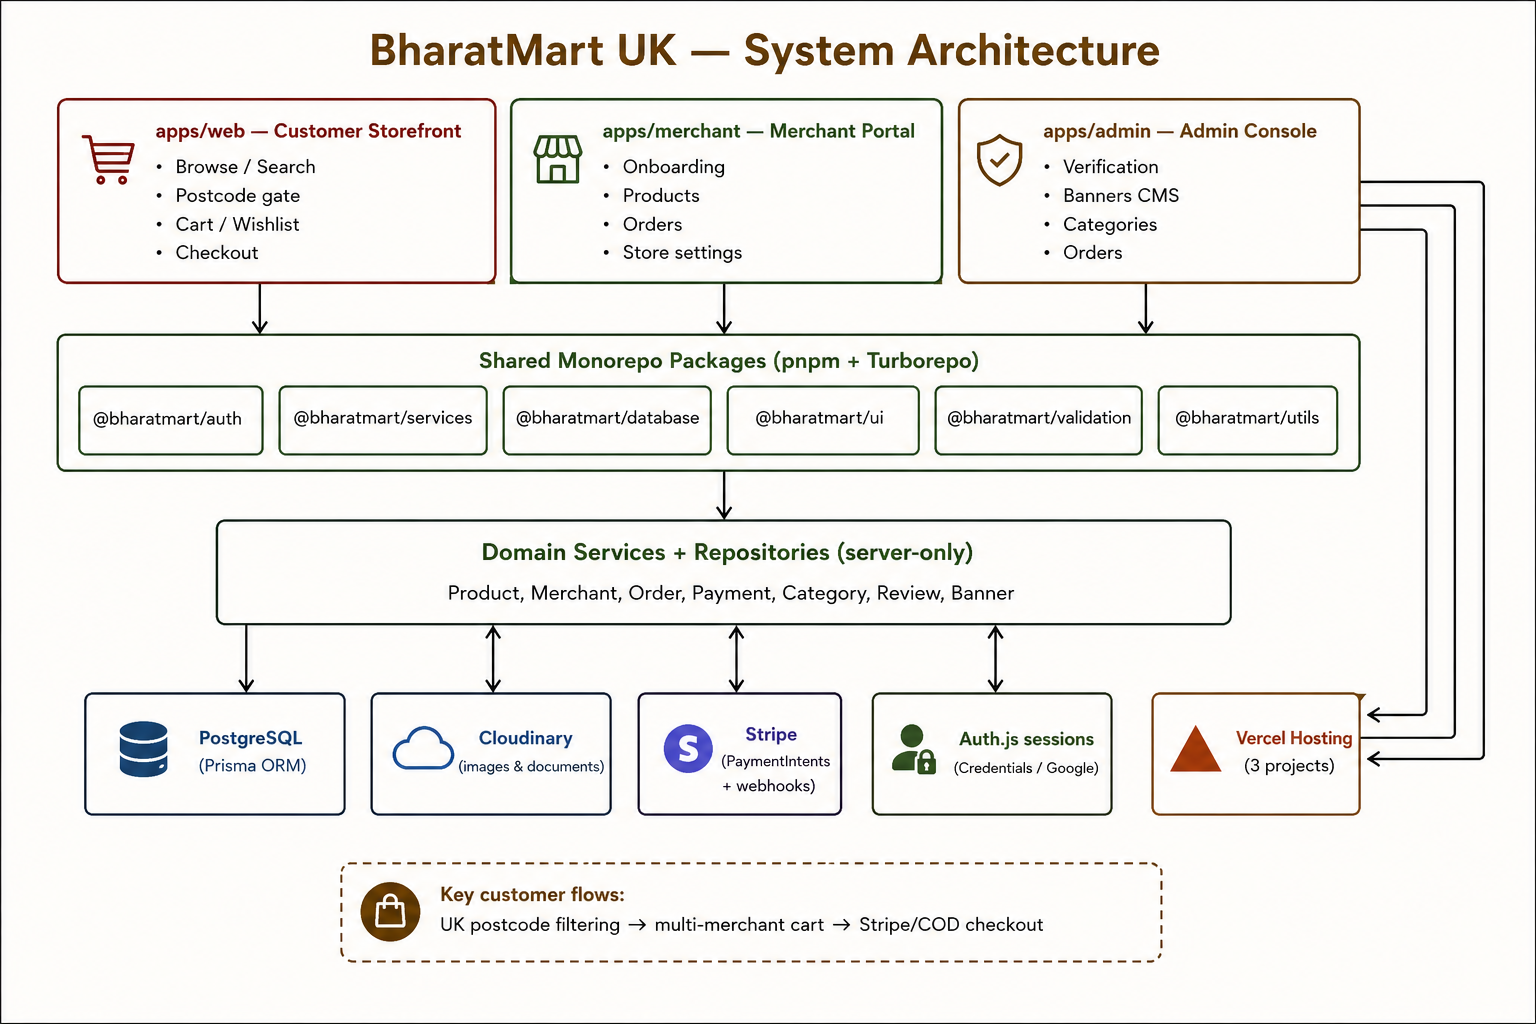
\includegraphics[width=0.9\textwidth]{Architecture.png}
    \caption{High-level monorepo architecture (Web / Merchant / Admin)}
    \label{fig:architecture}
\end{figure}


\section{Technology Stack}

Table~\ref{tab:tech_stack} summarises every major tool and framework used in
this project and the role it plays within the system.

\begin{table}[hbt!]
    \centering
    \renewcommand{\arraystretch}{1.35}
    \begin{tabular}{|p{3.5cm}|p{2.8cm}|p{6.5cm}|}
        \hline
        \textbf{Tool / Framework} & \textbf{Category} & \textbf{Role in the Project} \\
        \hline
        Next.js 15 & Web framework & App Router storefront, merchant, and admin apps \\
        \hline
        TypeScript & Language & End-to-end typed monorepo \\
        \hline
        Prisma + PostgreSQL & Data & Schema, migrations, and queries \\
        \hline
        Auth.js v5 & Auth & Credentials/Google; role-scoped sessions \\
        \hline
        Zod + RHF & Validation & Input schemas and form UX \\
        \hline
        Zustand & Client state & Cart and wishlist persistence \\
        \hline
        Stripe & Payments & PaymentIntents and webhook finalisation \\
        \hline
        Cloudinary & Media & Product, banner, logo, and document uploads \\
        \hline
        Turborepo + pnpm & Monorepo & Task orchestration and workspaces \\
        \hline
        Vercel & Hosting & Per-app production deployments \\
        \hline
        Tailwind + shared UI & Design system & Branded components and layout \\
        \hline
    \end{tabular}
    \vspace{0.2cm}
    \caption{Technology Stack and Roles}
    \label{tab:tech_stack}
\end{table}


\section{Domain Model and Data Layer}

Core entities include User, Merchant, Product, Category, Banner, Order,
MerchantOrder, Address, Coupon, and Review. Prices are stored in GBP pence.
Merchants declare \texttt{deliveryPostcodes}; product and merchant queries can
filter by customer postcode so the catalogue reflects deliverable sellers.
Checkout creates one customer Order that fans out into per-merchant
MerchantOrders for fulfilment.


\section{Customer Experience Design}

The first-visit experience optionally captures a UK postcode (soft gate with
skip). Logged-in users derive location from saved addresses. Search combines
autocomplete with heuristic fuzzy ranking (prefix/token/subsequence scoring)
and popularity-based recommendations when the query is empty. Product pages
expose Add to cart and Add to favourites rather than WhatsApp seller chat.

Figure~\ref{fig:journey} summarises the intended customer journey.

\begin{figure}[hbt!]
    \centering
    \includegraphics[width=0.9\textwidth]{customer_journey.png}
    \caption{Customer journey: Browse $\rightarrow$ Location $\rightarrow$ Cart $\rightarrow$ Checkout}
    \label{fig:journey}
\end{figure}


% CHAPTER 4
\chapter{IMPLEMENTATION AND DEPLOYMENT}

\section{Storefront Features Implemented}

Implemented storefront capabilities include homepage hero carousel
(CMS-driven banners), category grid, featured merchants, product listing with\\
filters/sort/pagination, product detail with image gallery, related products,
reviews listing, mobile navigation, wishlist page, account/address areas, and
info pages (About, Contact, Privacy, Terms).

\begin{figure}[hbt!]
    \centering
    \includegraphics[width=0.9\textwidth]{homepage.png}
    \caption{Storefront homepage composition (hero, categories, merchants)}
    \label{fig:homepage}
\end{figure}

\begin{figure}[hbt!]
    \centering
    \includegraphics[width=0.85\textwidth]{product_favourites.png}
    \caption{Product detail actions: Add to cart and Add to favourites}
    \label{fig:favourites}
\end{figure}


\section{Checkout, Payments, and Orders}

Checkout is a multi-step client flow (Address $\rightarrow$ Payment $\rightarrow$
Review). Payments support Stripe PaymentIntents and cash-on-delivery. On
successful payment webhook or COD confirmation, order finalisation creates
merchant sub-orders for fulfilment. Coupons can be validated on the cart.
Auth gates protect cart and wishlist actions with pending-action resume after
login.


\section{Search, Media, and Admin Support}

Header search calls a suggest API returning autocomplete or recommended
products. Product images and merchant documents are stored on Cloudinary rather
than the git repository. Admin tooling supports merchant verification review,
homepage carousel editing, category marketplace management, and order
inspection. Merchant tooling includes product CRUD, CSV bulk import, and
delivery postcode settings.

\begin{figure}[hbt!]
    \centering
    \includegraphics[width=0.85\textwidth]{postcode_gate.png}
    \caption{UK postcode gate and delivery filtering flow}
    \label{fig:postcode}
\end{figure}


\section{Deployment on Vercel}

Web, merchant, and admin deploy as separate Vercel projects sharing one
database. Production work included Prisma query-engine packaging in the
monorepo,\\ \texttt{AUTH\_SECRET}/Turbo environment passthrough, \texttt{AUTH\_URL}
cookie-prefix alignment to stop login bounce loops, ESLint rule registration
for Next.js, and Cloudinary-backed upload APIs suitable for serverless hosts.

The complete source code is publicly available at:

\vspace{0.2cm}
\begin{center}
{\small\textbf{GitHub Repository:}
\texttt{https://github.com/bharatmartuk/bharatmart-uk}}
\end{center}


% CHAPTER 5
\chapter{RESULTS AND EVALUATION}

\section{Deliverables Achieved}

Table~\ref{tab:deliverables} maps internship objectives to shipped outcomes.

\begin{table}[hbt!]
    \centering
    \renewcommand{\arraystretch}{1.45}
    \begin{tabular}{|p{4.2cm}|p{8.6cm}|}
        \hline
        \textbf{Objective} & \textbf{Delivered outcome} \\
        \hline
        Storefront UI/UX & Branded responsive marketplace with mobile navigation \\
        \hline
        Discovery & Catalogue, filters, fuzzy search, and recommendations \\
        \hline
        Delivery awareness & Postcode gate and merchant delivery filtering \\
        \hline
        Commerce & Cart, wishlist, multi-merchant checkout, Stripe/COD \\
        \hline
        Media \& CMS & Cloudinary assets; admin banner/category tools \\
        \hline
        Production & Vercel deployments; auth, media, and build fixes \\
        \hline
    \end{tabular}
    \vspace{0.2cm}
    \caption{Mapping of objectives to delivered features}
    \label{tab:deliverables}
\end{table}


\section{Qualitative Evaluation}

Success is evaluated qualitatively against internship goals: a working
end-to-end purchase path, coherent brand UX, deployable monorepo, and
demonstrable admin/merchant support. Git history from 18--22 July 2026 shows
intensive shipping culminating in production hardening; 23 July work extends
postcode UX and product favourites. The remaining week (24--30 July) is
reserved for QA and documentation close-out.

Limitations acknowledged: wishlist is client-persisted (Zustand) rather than
fully synced to a server Wishlist model; customer review write APIs are not
the focus of this internship slice; WhatsApp remains a support deep-link, not
a messaging API bot.


% CHAPTER 6
\chapter{CONCLUSION AND FUTURE ENHANCEMENTS}

\section{Conclusion}

This internship project successfully designed and implemented the BharatMart UK
customer marketplace as a production-oriented full-stack system. Working as a
\textbf{Full Stack Engineer Intern}, I owned UI/UX and engineering for
discovery, location-aware browsing, cart/wishlist, checkout/payments, and
deployment polish within a shared monorepo architecture.

The experience provided end-to-end ownership of a real commerce product ---
from interface composition and domain modelling to third-party integrations and
cloud deployment --- strengthening readiness for industry software roles.


\section{Future Enhancements}

The following enhancements are identified for further development of the
system:

\begin{itemize}
    \item \textbf{Server-synced wishlist} --- Persist favourites and followed
    stores using existing Prisma models rather than client-only state.
    \item \textbf{Customer review submission} --- Add write and moderation
    workflows for product reviews.
    \item \textbf{Stronger personalisation} --- Introduce learned ranking or
    embeddings on top of the current fuzzy search heuristics.
    \item \textbf{Merchant coupon management UI} --- Complement cart-side
    coupon validation with seller-facing coupon tools.
    \item \textbf{Automated end-to-end tests} --- Cover checkout and postcode
    filtering in continuous integration.
    \item \textbf{Expanded merchant analytics} --- Extend dashboards beyond
    current revenue charts.
\end{itemize}


% REFERENCES
\chapter*{REFERENCES}
\addcontentsline{toc}{chapter}{References}

\begin{enumerate}

    \item BharatMart.uk marketplace source code.
    \\
    \texttt{https://github.com/bharatmartuk/bharatmart-uk}

    \item BharatMart.uk product website.
    \texttt{https://bharatmart.uk}

    \item Next.js Documentation, Vercel.
    \texttt{https://nextjs.org/docs}

    \item Prisma ORM Documentation.
    \texttt{https://www.prisma.io/docs}

    \item Auth.js Documentation.
    \texttt{https://authjs.dev}

    \item Stripe Payment Intents Documentation.\\
    \texttt{https://docs.stripe.com/payments/payment-intents}

    \item Cloudinary Upload API Documentation.\\
    \texttt{https://cloudinary.com/documentation}

    \item Turborepo Documentation.
    \texttt{https://turbo.build/repo/docs}

    \item Vercel Deployment Documentation.
    \texttt{https://vercel.com/docs}

    \item Tailwind CSS Documentation.
    \texttt{https://tailwindcss.com/docs}

\end{enumerate}

\end{document}
